\documentclass[journal]{IEEEtran}

% ============================================================================
% PAQUETES
% ============================================================================
\usepackage[utf8]{inputenc}
\usepackage[T1]{fontenc}
\usepackage[spanish]{babel}
\addto\captionsspanish{\renewcommand{\abstractname}{Resumen}}
\usepackage{graphicx}
\usepackage{amsmath}
\usepackage{array}
\usepackage{float}
\usepackage{url}
\usepackage{listings}
\usepackage{xcolor}
\usepackage{booktabs}
\usepackage{multirow}
\usepackage{hyperref}
\usepackage{caption}
\usepackage{subcaption}
\usepackage{longtable}
\usepackage{pdflscape}

% ============================================================================
% CONFIGURACIÓN DE CÓDIGO
% ============================================================================
\lstset{
  backgroundcolor=\color{gray!10},
  basicstyle=\ttfamily\footnotesize,
  breaklines=true,
  frame=single,
  numbers=left,
  numberstyle=\tiny\color{gray},
  keywordstyle=\color{blue},
  commentstyle=\color{green!50!black},
  stringstyle=\color{orange},
  captionpos=b,
  tabsize=2
}

% ============================================================================
% DATOS DEL DOCUMENTO
% ============================================================================
\title{
CrowdStrike Falcon Alert Simulator:\\
Primera Entrega --- Aplicación Web Pública por HTTP
}

\author{
Brayan Loaiza Leal,
Juan Sebastián Guayazán Clavijo
\thanks{Fundamentos de Seguridad de la Información (ISIS FDSI-4L)}
\thanks{Ingeniería de Sistemas}
\thanks{Escuela Colombiana de Ingeniería Julio Garavito}
\thanks{2026-2, Segundo Tercio}
}

\markboth{
Laboratorio 03 --- Red Team vs. Blue Team
}{
CrowdStrike Falcon Alert Simulator
}

% ============================================================================
% DOCUMENTO
% ============================================================================
\begin{document}

\maketitle

% ============================================================================
% RESUMEN
% ============================================================================
\begin{abstract}
Este documento presenta la primera entrega del Laboratorio 03 de Fundamentos
de Seguridad de la Información, correspondiente al reto Secure Product
Challenge. El equipo seleccionó la Opción 1 (automatización de incidentes de
CrowdStrike Falcon) y desarrolló un prototipo denominado \textit{CrowdStrike
Falcon Alert Simulator}: dos microservicios Flask (\texttt{alerts-api} y
\texttt{actions-api}) que simulan la recepción, consulta y registro de
acciones sobre alertas ficticias de seguridad, junto con un dashboard estático
servido por Nginx. La primera versión establece una línea base deliberadamente
insegura y controlada --- HTTP sin TLS, sin autenticación --- utilizando
únicamente información ficticia, desplegada sobre una VM Ubuntu Server
26.04.1 LTS en VMware Workstation. El trabajo comprende la descripción del
problema, la arquitectura implementada, la estructura del repositorio, las
evidencias de ejecución local y del servidor, un fallo real de despliegue
encontrado y corregido (bloqueo por CORS entre el dashboard y la API), y un
modelo inicial de amenazas STRIDE con una hipótesis por cada una de las seis
categorías, derivada directamente del código fuente de los microservicios.
Las pruebas y evidencias presentadas se limitan al entorno autorizado para el
laboratorio y utilizan exclusivamente datos ficticios.
\end{abstract}

\begin{IEEEkeywords}
HTTP, Nginx, Flask, Red Team, Blue Team, STRIDE, Threat Modeling,
CrowdStrike Falcon, microservicios, Ubuntu Server.
\end{IEEEkeywords}

\IEEEpeerreviewmaketitle

% ============================================================================
% 1. PORTADA Y DATOS DEL EQUIPO
% ============================================================================
% Cubierto por \maketitle (título, autores, afiliación, fecha del tercio).

% ============================================================================
% 2. DESCRIPCIÓN DEL PROYECTO
% ============================================================================
\section{Descripción del Proyecto}

\subsection{Problema seleccionado}

Opción 1: automatización de incidentes de CrowdStrike Falcon. La recepción,
clasificación, enriquecimiento y escalamiento de alertas de seguridad suele
requerir actividades manuales que aumentan el tiempo de respuesta, dificultan
la correlación de evidencias y generan criterios distintos al priorizar
incidentes. Para este laboratorio se seleccionó la construcción de un
prototipo denominado \textit{CrowdStrike Falcon Alert Simulator}, diseñado
exclusivamente para fines académicos y utilizando información completamente
ficticia, sin integración real con la API de CrowdStrike.

\subsection{Objetivo de la primera versión}

Construir y publicar, mediante HTTP y sin autenticación, un prototipo que
reciba alertas ficticias de CrowdStrike Falcon, permita consultarlas mediante
una API REST y registre las acciones de respuesta ejecutadas por analistas.
Esta versión establece una línea base técnica y una superficie controlada
para las posteriores actividades de Red Team y Blue Team.

\subsection{Usuarios previstos}

Analistas SOC (Blue Team) que consultan el dashboard y registran acciones de
respuesta sobre las alertas; el equipo Red Team, que ejercerá reconocimiento
autorizado (Nmap, curl, ZAP) sobre la superficie expuesta en la Parte II desde
una estación Kali Linux.

\subsection{Datos ficticios}

El prototipo utiliza únicamente información creada para el laboratorio:

\begin{itemize}
    \item Cinco alertas precargadas (\texttt{ALT-001}--\texttt{ALT-005}):
    malware, movimiento lateral, escalamiento de privilegios, fuerza bruta y
    exfiltración de datos.
    \item Tres acciones de analista precargadas (\texttt{ACT-001}--\texttt{ACT-003}).
    \item Usuarios y hosts ficticios: \texttt{john.doe}, \texttt{jane.smith},
    \texttt{carlos.garcia}, \texttt{maria.torres}, \texttt{contractor01};
    \texttt{WORKSTATION-42}, \texttt{SERVER-DC01}, entre otros.
\end{itemize}

No se utilizan credenciales, tokens, información personal, direcciones
internas reales ni información perteneciente a sistemas de producción.

\subsection{Alcance y exclusiones}

El alcance de esta primera versión comprende:

\begin{itemize}
    \item Dos microservicios REST en Flask (\texttt{alerts-api} en el puerto
    5000, \texttt{actions-api} en el puerto 5001).
    \item Un dashboard estático servido por Nginx que consume ambas APIs.
    \item Publicación mediante Nginx sobre Ubuntu Server, protocolo HTTP sobre
    el puerto TCP 80, con proxy inverso hacia los microservicios.
    \item Registro de eventos mediante los logs de Nginx y de cada
    microservicio.
    \item Documentación de la arquitectura, los flujos de información y la
    estructura del repositorio.
    \item Elaboración de un modelo inicial de amenazas mediante STRIDE (seis
    categorías).
\end{itemize}

Se excluyen de esta versión: información real, autenticación y autorización,
HTTPS/TLS (Laboratorio 4), persistencia en base de datos (los datos viven en
memoria), integración real con la API de CrowdStrike, explotación destructiva,
denegación de servicio, fuerza bruta, persistencia, y las rondas activas de
Red/Blue Team con Nmap, ZAP, tcpdump y hardening formal, que corresponden a la
Parte II de este mismo laboratorio.

\subsection{Resultado esperado del despliegue}

Al finalizar esta primera versión se dispone de un prototipo accesible desde
la VM del laboratorio mediante HTTP, con Nginx y los dos microservicios
correctamente configurados como servicios \texttt{systemd}, registros de
acceso y errores disponibles para su análisis, una arquitectura documentada
(incluyendo un hallazgo real de diseño corregido) y un modelo inicial de
amenazas que sirve de línea base para las siguientes fases del reto.

% ============================================================================
% 3. ARQUITECTURA IMPLEMENTADA
% ============================================================================
\section{Arquitectura Implementada}

La arquitectura implementada corresponde a dos microservicios Flask sin
autenticación, un dashboard estático y un proxy Nginx, publicados por HTTP
sobre una VM Ubuntu Server. La estación Kali Linux representará, en la
Parte II, el entorno desde el cual se realizan las pruebas autorizadas de
Red Team; el Blue Team observará el comportamiento del servidor mediante sus
registros.

\subsection{Actores}

\begin{itemize}
    \item \textbf{Analista SOC / Blue Team:} consulta el dashboard y registra
    acciones de respuesta.
    \item \textbf{Red Team / Kali (Parte II):} realiza reconocimiento y
    pruebas autorizadas (Nmap, curl, ZAP).
    \item \textbf{Cliente HTTP anónimo:} cualquier origen en la red del
    laboratorio; no existe distinción de privilegio porque no hay
    autenticación.
    \item \textbf{Administrador/Builder:} mantiene el repositorio, el servidor
    y la configuración de Nginx.
\end{itemize}

\subsection{Componentes}

\begin{itemize}
    \item Nginx (proxy inverso y contenido estático, puerto 80).
    \item \texttt{alerts-api} --- microservicio Flask (puerto 5000).
    \item \texttt{actions-api} --- microservicio Flask (puerto 5001).
    \item Dashboard estático (\texttt{frontend/index.html}).
    \item Registros \texttt{lab3\_access.log}, \texttt{lab3\_error.log}
    (Nginx), \texttt{alerts.log}, \texttt{actions.log} (Flask).
\end{itemize}

\subsection{Flujos de datos}

\begin{center}
\textbf{Navegador}
$\rightarrow$
\textbf{Nginx (:80)}
$\rightarrow$
\textbf{proxy\_pass /api/alerts/ y /api/actions/}
$\rightarrow$
\textbf{alerts-api (:5000) / actions-api (:5001)}
\end{center}

\textbf{Hallazgo de arquitectura corregido durante esta entrega:} el
JavaScript del dashboard llamaba originalmente de forma directa a
\texttt{http://<host>:5000}, evitando el proxy de Nginx. Al desplegar en la VM
real se detectó que esa llamada cruzada de puerto era bloqueada por CORS en el
navegador (Flask no envía \texttt{Access-Control-Allow-Origin}), mientras que
\texttt{curl} sí funcionaba, ocultando el problema en pruebas de servidor a
servidor. Se corrigió \texttt{frontend/index.html} para consumir la API vía
el proxy (\texttt{/api/alerts/alerts}), quedando \textit{same-origin}; el
retest con captura de navegador confirma la corrección (Sección
\ref{sec:evidencia-servidor}).

\subsection{Almacenes de datos}

El prototipo no usa base de datos: los datos viven en listas de Python en
memoria dentro de cada microservicio, sin persistencia entre reinicios.

\begin{lstlisting}
ALERTS  -> lista en memoria (alerts-api)
ACTIONS -> lista en memoria (actions-api)
\end{lstlisting}

Los registros del servidor constituyen la fuente de trazabilidad:

\begin{lstlisting}[language=bash]
/var/log/nginx/lab3_access.log
/var/log/nginx/lab3_error.log
services/alerts-api/alerts.log
services/actions-api/actions.log
\end{lstlisting}

\subsection{Protocolo y puertos}

\begin{table}[H]
\centering
\caption{Protocolos y puertos principales}
\label{tab:protocolos}
\begin{tabular}{|p{2.7cm}|p{1.6cm}|p{2cm}|}
\hline
\textbf{Servicio} & \textbf{Protocolo} & \textbf{Puerto} \\
\hline
Nginx (proxy + estático) & HTTP & TCP/80 \\
\hline
alerts-api (Flask, bind 0.0.0.0) & HTTP & TCP/5000 \\
\hline
actions-api (Flask, bind 0.0.0.0) & HTTP & TCP/5001 \\
\hline
Administración del servidor & SSH & TCP/22 \\
\hline
\end{tabular}
\end{table}

Los puertos 5000/5001 quedan expuestos directamente en la red (bind
\texttt{0.0.0.0}), no solo tras el proxy --- un hallazgo relevante para el
modelo de amenazas (Sección \ref{sec:amenazas}).

\subsection{Límites de confianza}

\begin{enumerate}
    \item \textbf{L1:} frontera entre la red del laboratorio/Internet y Nginx.
    \item \textbf{L2:} frontera entre Nginx y los microservicios Flask;
    debilitada porque ambos hacen bind en \texttt{0.0.0.0} y son alcanzables
    directamente, sin pasar por Nginx.
    \item \textbf{L3:} frontera entre el navegador y la API consumida por el
    dashboard --- corregida en esta entrega para que pase por el proxy
    (same-origin) en vez de saltárselo.
\end{enumerate}

\subsection{Punto de generación de logs}

Nginx registra en \texttt{lab3\_access.log} la IP de origen, fecha y hora,
método, ruta, código de respuesta y User-Agent de cada solicitud; los errores
del servicio quedan en \texttt{lab3\_error.log}. Cada microservicio Flask
registra en su propio archivo (\texttt{alerts.log}, \texttt{actions.log}) las
solicitudes y respuestas mediante los manejadores \texttt{before\_request} /
\texttt{after\_request}.

\subsection{Diagrama de arquitectura y flujo de datos}

La Figura~\ref{fig:arquitectura} presenta la arquitectura implementada,
identificando actores, componentes, protocolo, puertos, almacenes de datos,
límites de confianza y puntos de generación de logs.

\begin{figure}[H]
    \centering
    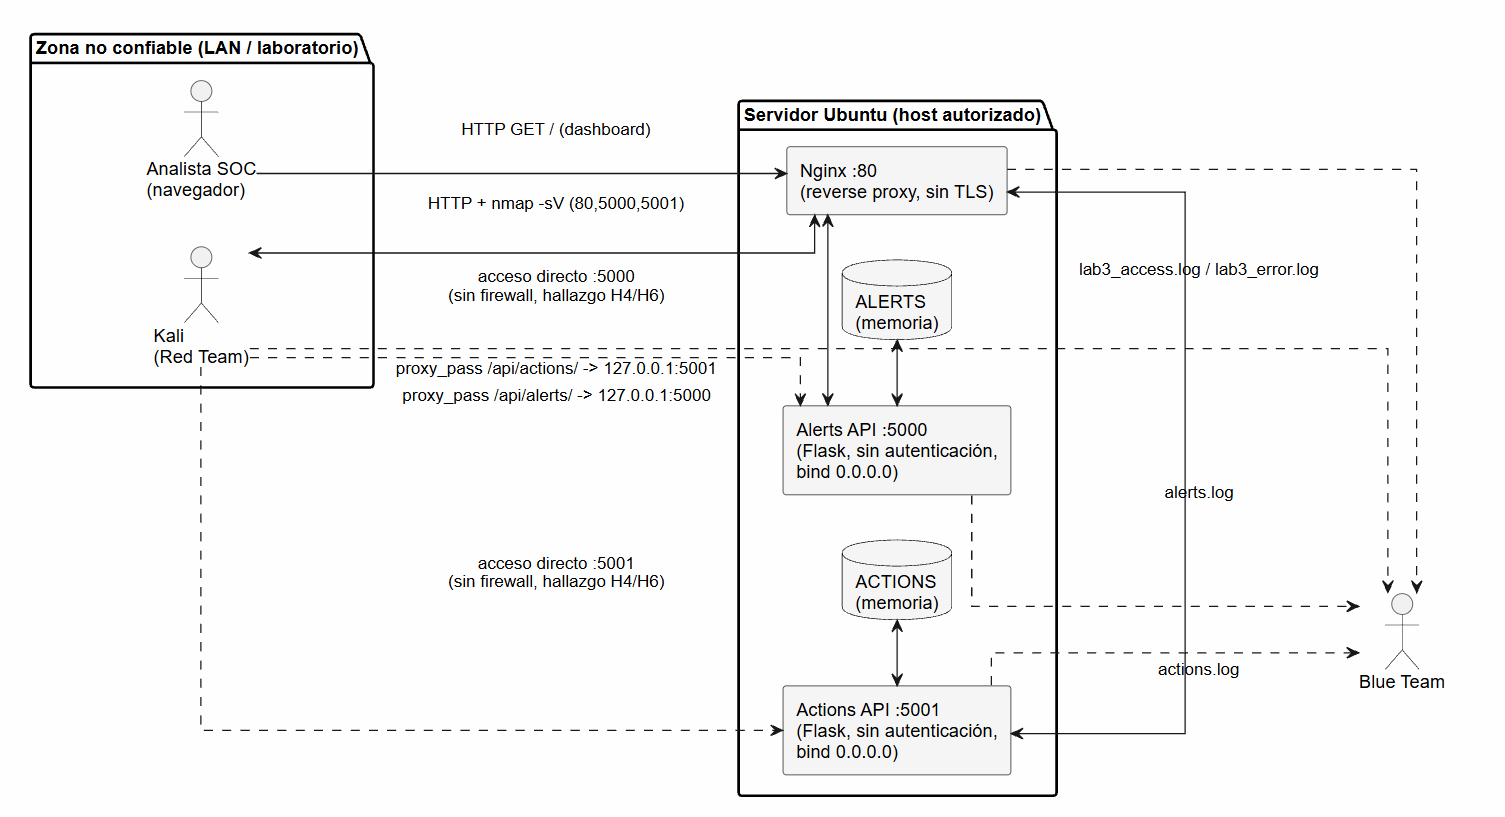
\includegraphics[width=\columnwidth]{images/dfd-lab3}
    \caption{Diagrama de Flujo de Datos --- CrowdStrike Falcon Alert Simulator.}
    \label{fig:arquitectura}
\end{figure}
% PENDIENTE: exportar el diagrama (artifact Mermaid) como PNG y subirlo a
% images/dfd-lab3.png en el proyecto de Overleaf.

% ============================================================================
% 4. ESTRUCTURA DEL REPOSITORIO
% ============================================================================
\section{Estructura del Repositorio}

El repositorio
\url{https://github.com/BrayanLoaiza-JuanGuayazan-FDSI/Lab3-FDSI} sigue la
siguiente estructura:

\begin{lstlisting}
Lab3-FDSI/
|-- frontend/index.html
|-- nginx/lab3-fdsi.conf
|-- services/
|   |-- alerts-api/  (app.py, requirements.txt)
|   `-- actions-api/ (app.py, requirements.txt)
|-- diagrams/dfd-lab3.png
|-- evidence/{local-exec.txt,server-nginx.txt,red/,blue/}
|-- reports/zap-passive/
|-- risk-register.md
|-- threat-model/threat-model.xlsx
|-- deploy.sh
`-- README.md
\end{lstlisting}

El \texttt{README.md} documenta: propósito del proyecto, arquitectura,
requisitos (Ubuntu 20.04+, Python 3.8+, Nginx, pip3), ejecución local,
procedimiento de despliegue mediante \texttt{deploy.sh}, la URL publicada
(\texttt{http://192.168.17.129/}), los integrantes del equipo y las
limitaciones de seguridad conocidas (sin autenticación, sin TLS,
\texttt{/debug/env} expuesto, sin validación de entrada, sin rate limiting,
sin cabeceras de seguridad, datos en memoria, logs sin cifrar). El
\texttt{risk-register.md} contiene activos, actores, límites de confianza y
superficie de ataque; la matriz de hipótesis STRIDE y de mitigaciones vive en
\texttt{threat-model/threat-model.xlsx}.

% ============================================================================
% 5. EVIDENCIAS DE EJECUCIÓN LOCAL
% ============================================================================
\section{Evidencias de Ejecución Local}

La ejecución local permite comprobar que el repositorio fue clonado
correctamente, que los archivos de la aplicación existen y que el frontend
funciona antes del despliegue en el servidor. El comando exacto usado en cada
prueba se lista en el Anexo~\ref{app:comandos}.

\subsection{Estado del repositorio}

\begin{figure}[H]
    \centering
    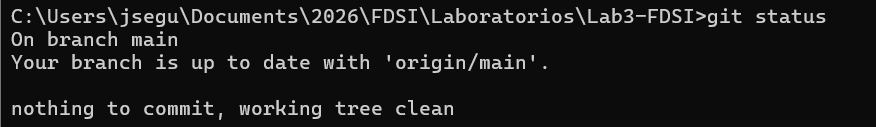
\includegraphics[width=\columnwidth]{images/git-status}
    \caption{Estado del repositorio mediante \texttt{git status}.}
    \label{fig:git_status}
\end{figure}
% Salida real de referencia: "On branch main, up to date with origin/main,
% nothing to commit, working tree clean" (tras subir los commits de esta entrega).

\subsection{Historial de commits}

\begin{figure}[H]
    \centering
    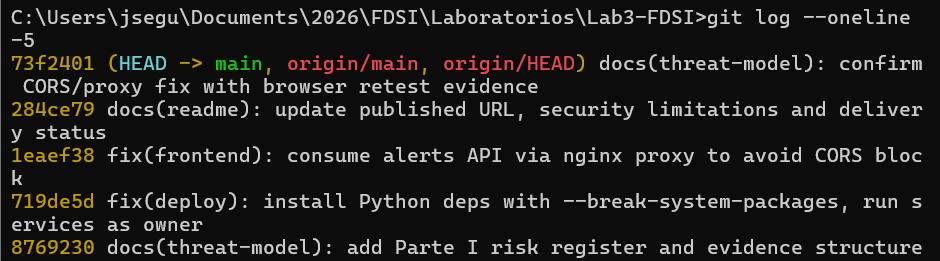
\includegraphics[width=\columnwidth]{images/git-log}
    \caption{Últimos cinco commits del repositorio.}
    \label{fig:git_log}
\end{figure}
% PENDIENTE: el historial siguio cambiando (informe y threat-model.xlsx se
% agregaron despues de tomar la captura images/git-log.png); volver a ejecutar
% "git log --oneline -5" en el repositorio ya actualizado y reemplazar la
% captura antes de compilar. Salida real de referencia (2026-09-14):
% dfac8e8 docs(threat-model): move STRIDE matrix and mitigations from report to xlsx
% a2fb793 docs(report): move executed commands to appendix, keep only results in body
% df143a0 fix(report): widen deployment diagnostics table to span both columns
% a8193b2 docs(report): add IEEE writeup for Parte I
% 83de96a docs(threat-model): confirm CORS/proxy fix with browser retest evidence

\subsection{Archivos del proyecto}

\begin{figure}[H]
    \centering
    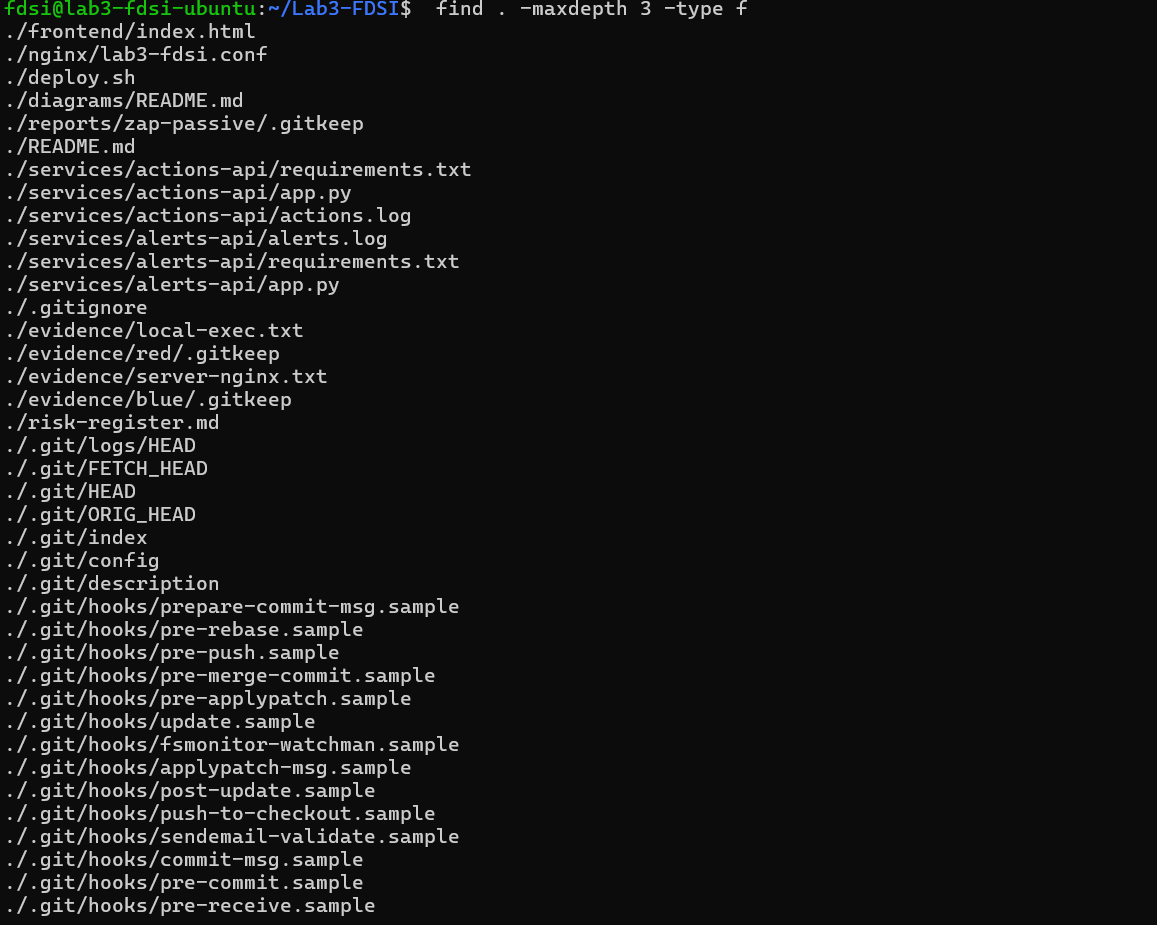
\includegraphics[width=\columnwidth]{images/find-files}
    \caption{Archivos presentes en el repositorio.}
    \label{fig:find_files}
\end{figure}
% Debe evidenciar, entre otros: frontend/index.html, nginx/lab3-fdsi.conf,
% services/alerts-api/app.py, services/actions-api/app.py, risk-register.md.

\subsection{Servidor HTTP local}

Se sirvió \texttt{frontend/index.html} con \texttt{python3 -m http.server 8080}
y se verificó con \texttt{curl -I}/\texttt{curl} contra \texttt{localhost:8080}
(comandos completos en el Anexo~\ref{app:comandos}). Respuesta obtenida:

\begin{lstlisting}
HTTP/1.0 200 OK
Server: SimpleHTTP/0.6 Python/3.14.0
Date: Mon, 14 Sep 2026 11:18:38 GMT
Content-type: text/html
Content-Length: 8294
\end{lstlisting}

El cuerpo de la respuesta contiene el \texttt{<title>Falcon Alerts</title>} del
dashboard, confirmando que \texttt{index.html} existe y se sirve correctamente
de forma local antes del despliegue en el servidor.

% PENDIENTE: esta captura es "curl -I http://localhost/" contra Nginx en la
% VM (puerto 80) -- es la misma prueba que la Figura de la Seccion 6
% (curl-nginx). Reemplazar por una captura real de
% "python3 -m http.server 8080" + "curl -I http://localhost:8080" en la
% maquina de desarrollo, que es la evidencia que pide la rubrica en esta
% subseccion.
\begin{figure}[H]
    \centering
    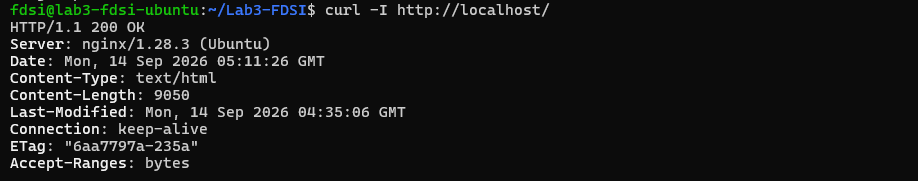
\includegraphics[width=\columnwidth]{images/curl-local}
    \caption{Prueba de disponibilidad del frontend con \texttt{python3 -m http.server 8080} (HTTP 200).}
    \label{fig:curl_local}
\end{figure}

\subsection{Fecha y hora de las pruebas}

Obtenida con \texttt{date -u +\%Y-\%m-\%dT\%H:\%M:\%SZ}.
Evidencia de ejecución local: \texttt{2026-09-14T11:18:38Z}. Evidencia de
despliegue en servidor: \texttt{2026-09-14T03:48:11Z}.

% ============================================================================
% 6. EVIDENCIAS DEL SERVIDOR Y NGINX
% ============================================================================
\section{Evidencias del Servidor y Nginx}
\label{sec:evidencia-servidor}

Servidor: VM Ubuntu Server 26.04.1 LTS en VMware Workstation (red NAT), host
\texttt{lab3-fdsi-ubuntu}, IP \texttt{192.168.17.129}. Los comandos exactos
usados en esta sección se listan en el Anexo~\ref{app:comandos}.

\subsection{Identificación del servidor}

\begin{figure}[H]
    \centering
    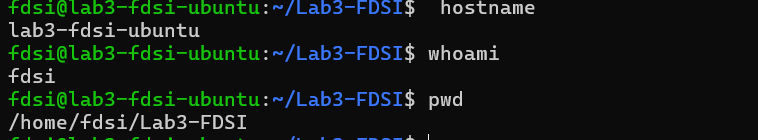
\includegraphics[width=\columnwidth]{images/server-baseline}
    \caption{Identificación y línea base del servidor.}
    \label{fig:server_baseline}
\end{figure}

\subsection{Versión de Nginx}

Obtenida con \texttt{nginx -v}: \texttt{nginx/1.28.3 (Ubuntu)}.

\subsection{Estado del servicio}

\begin{figure}[H]
    \centering
    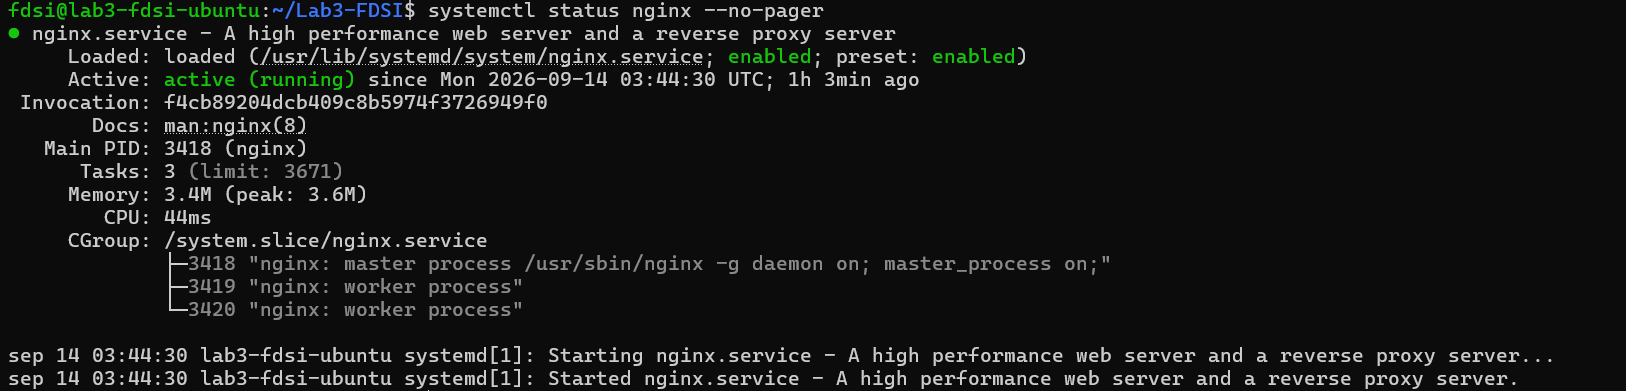
\includegraphics[width=\columnwidth]{images/nginx-status}
    \caption{Estado del servicio Nginx (\texttt{active/running}).}
    \label{fig:nginx_status}
\end{figure}

\subsection{Validación de la configuración}

Resultado de \texttt{sudo nginx -t}:
\begin{lstlisting}
nginx: the configuration file /etc/nginx/nginx.conf syntax is ok
nginx: configuration file /etc/nginx/nginx.conf test is successful
\end{lstlisting}

\subsection{Prueba HTTP local}

Verificada con \texttt{curl -I} sobre el frontend (:80) y el health check de
cada microservicio (:5000, :5001):

\begin{figure}[H]
    \centering
    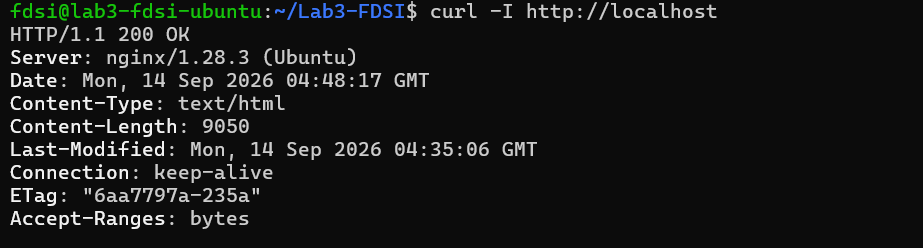
\includegraphics[width=\columnwidth]{images/curl-nginx}
    \caption{Respuesta HTTP generada por Nginx (200 OK).}
    \label{fig:curl_nginx}
\end{figure}
Código HTTP obtenido en los tres casos: \texttt{200 OK}.

\subsection{Configuración del servidor}

El virtual host utilizado corresponde a:

\begin{lstlisting}[language=bash]
server {
    listen 80;
    server_name _;

    access_log /var/log/nginx/lab3_access.log;
    error_log  /var/log/nginx/lab3_error.log;

    root /var/www/lab3;
    index index.html;

    location / {
        try_files $uri $uri/ /index.html;
    }

    location /api/alerts/ {
        proxy_pass http://127.0.0.1:5000/;
        proxy_set_header Host $host;
        proxy_set_header X-Real-IP $remote_addr;
    }

    location /api/actions/ {
        proxy_pass http://127.0.0.1:5001/;
        proxy_set_header Host $host;
        proxy_set_header X-Real-IP $remote_addr;
    }
}
\end{lstlisting}

\subsection{Permisos del directorio publicado}

Resultado de \texttt{ls -la /var/www/lab3}:
\begin{lstlisting}
drwxr-xr-x 2 root root 4096 Sep 14 03:41 .
-rwxr-xr-x 1 root root 9083 Sep 14 03:44 index.html
\end{lstlisting}

Los archivos son propiedad de \texttt{root} con permisos \texttt{755}/\texttt{755},
legibles y ejecutables (traversal de directorio) por Nginx sin otorgar permiso
de escritura al proceso del servidor web.

\subsection{Access log}

Extracto de \texttt{sudo tail -n 50 /var/log/nginx/lab3\_access.log}:

\begin{figure}[H]
    \centering
    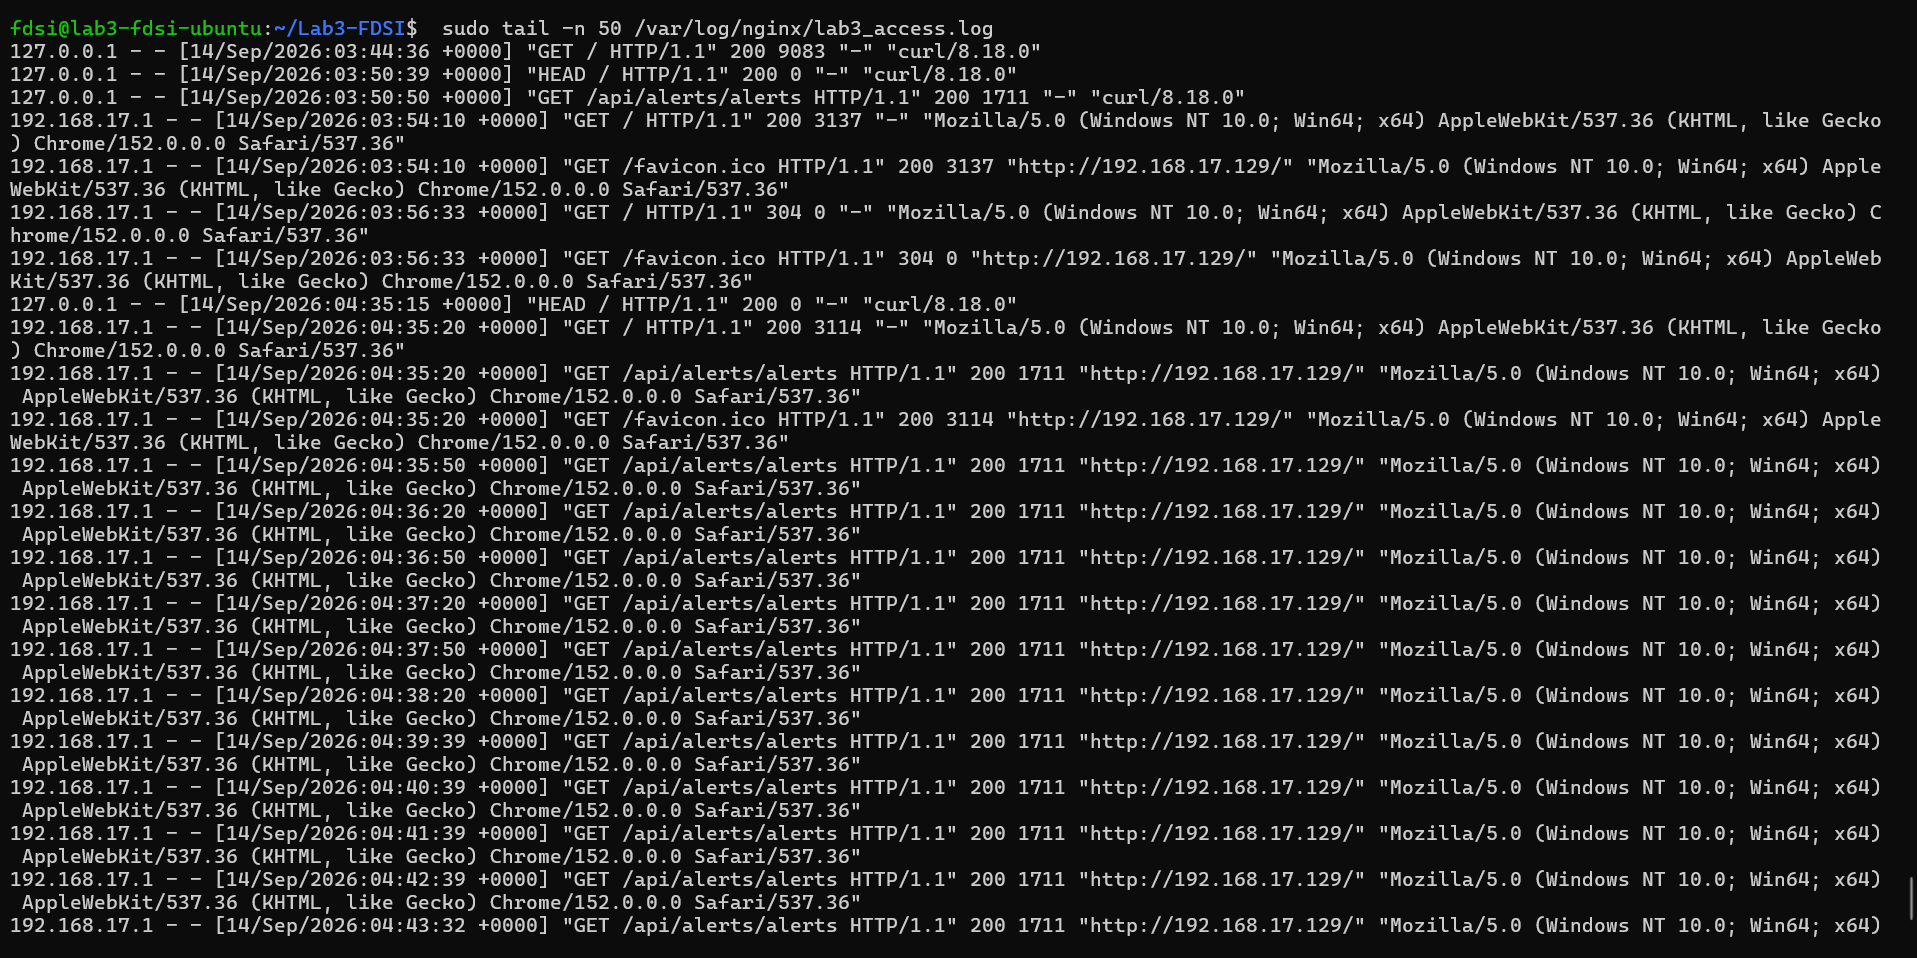
\includegraphics[width=\columnwidth]{images/access-log}
    \caption{Extracto del registro de acceso de Nginx --- incluye tráfico real
    del navegador (\texttt{192.168.17.1}) consumiendo \texttt{/api/alerts/alerts}
    cada 30 segundos, correspondiente al refresco automático del dashboard.}
    \label{fig:access_log}
\end{figure}

\subsection{Error log}

Extracto de \texttt{sudo tail -n 30 /var/log/nginx/lab3\_error.log}:

\begin{figure}[H]
    \centering
    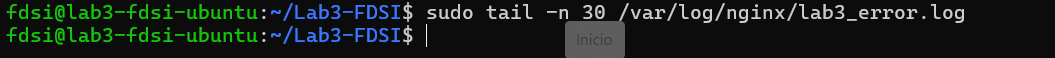
\includegraphics[width=\columnwidth]{images/error-log}
    \caption{Registro de errores de Nginx (vacío, sin errores registrados).}
    \label{fig:error_log}
\end{figure}

\subsection{Captura del navegador}

La Figura~\ref{fig:browser} muestra el dashboard accedido desde
\texttt{http://192.168.17.129/}, con las cinco alertas y los contadores por
severidad correctamente cargados tras la corrección del bloqueo por CORS
descrita en la Sección~\ref{sec:amenazas} (hallazgo L3).

% PENDIENTE: esta captura corresponde a la version anterior del dashboard,
% con el titulo "CrowdStrike Falcon Simulator" y el banner de advertencia de
% laboratorio. El frontend fue simplificado (sin ese texto); volver a tomar
% la captura contra el servidor ya redesplegado antes de compilar.
\begin{figure}[H]
    \centering
    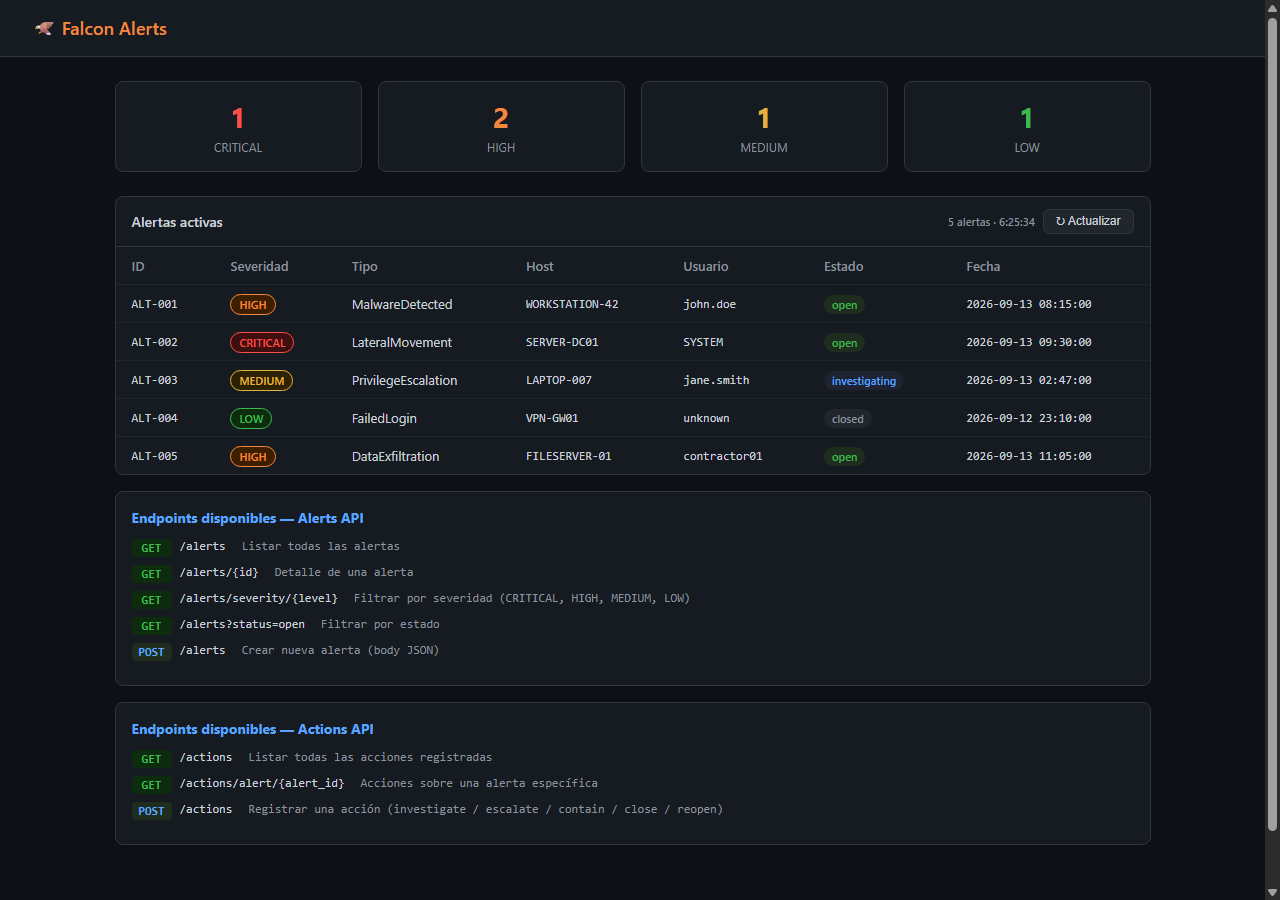
\includegraphics[width=\columnwidth]{images/browser-dashboard}
    \caption{Dashboard de alertas cargado correctamente, 5 alertas
    (1 CRITICAL, 2 HIGH, 1 MEDIUM, 1 LOW).}
    \label{fig:browser}
\end{figure}

% ============================================================================
% 7. DIAGNÓSTICO DEL FALLO
% ============================================================================
\section{Diagnóstico del Fallo}

El despliegue se completó exitosamente; no obstante, durante el proceso se
presentaron dos fallos reales, diagnosticados y corregidos, que se documentan
por su valor metodológico.

\begin{table*}[t]
\centering
\caption{Diagnóstico de problemas durante el despliegue}
\label{tab:diagnostico}
\small
\renewcommand{\arraystretch}{1.3}
\begin{tabular}{|>{\raggedright\arraybackslash}p{3.2cm}|>{\raggedright\arraybackslash}p{2.6cm}|>{\raggedright\arraybackslash}p{4.5cm}|>{\raggedright\arraybackslash}p{6.5cm}|}
\hline
\textbf{Prueba} &
\textbf{Esperado} &
\textbf{Obtenido} &
\textbf{Diagnóstico} \\
\hline
curl localhost & HTTP 200 & HTTP 200 & OK, sin fallo \\
\hline
nginx -t & Syntax OK & Syntax OK & OK, sin fallo \\
\hline
\texttt{pip3 install} & Instalación OK & \texttt{externally-managed-environment} & Python 3.14/Ubuntu 26.04 (PEP 668); corregido con \texttt{--break-system-packages} \\
\hline
Arranque \texttt{alerts-api}/\texttt{actions-api} & \texttt{active (running)} & \texttt{status=200/CHDIR} & \texttt{User=www-data} sin permiso sobre \texttt{\$HOME} (750); corregido a usuario dueño del repo \\
\hline
Carga del dashboard & Alertas visibles & \texttt{Error conectando a la API} & CORS: fetch cruzado de puerto bloqueado; corregido consumiendo vía proxy Nginx \\
\hline
\end{tabular}
\end{table*}

Los tres últimos casos están documentados en detalle, con evidencia de
comando/log y corrección aplicada, en \texttt{risk-register.md} y en las
secciones anteriores de este informe.

% ============================================================================
% 8. MODELO DE AMENAZAS INICIAL
% ============================================================================
\section{Modelo de Amenazas Inicial}
\label{sec:amenazas}

El modelo de amenazas permite identificar los activos, actores, límites de
confianza y posibles riesgos de seguridad existentes en la primera versión
del sistema. El detalle narrativo se encuentra en \texttt{risk-register.md};
la matriz de amenazas STRIDE y de mitigaciones, en
\texttt{threat-model/threat-model.xlsx}.

\subsection{Activos}

\begin{itemize}
    \item Datos de alertas (\texttt{ALERTS}) y de acciones (\texttt{ACTIONS}).
    \item Código fuente del repositorio.
    \item Configuración de Nginx y procesos \texttt{alerts-api}/\texttt{actions-api}.
    \item Registros (\texttt{lab3\_access.log}, \texttt{lab3\_error.log},
    \texttt{alerts.log}, \texttt{actions.log}).
    \item El host (VM Ubuntu Server).
\end{itemize}

\subsection{Actores}

Analista SOC (Blue Team); Red Team / Kali (Parte II); cliente HTTP anónimo (sin
distinción de privilegio); administrador/Builder con acceso \texttt{sudo}.

\subsection{Límites de confianza}

Ver Sección~\ref{sec:amenazas} de Arquitectura: L1 (Internet/LAN
$\rightarrow$ Nginx), L2 (Nginx $\rightarrow$ microservicios Flask, debilitado
por bind \texttt{0.0.0.0}) y L3 (navegador $\rightarrow$ API, corregido en
esta entrega).

\subsection{Superficie de ataque}

\begin{itemize}
    \item Puertos TCP 80, 5000 y 5001 expuestos.
    \item Endpoints enumerables sin autenticación: \texttt{/alerts},
    \texttt{/alerts/\{id\}}, \texttt{/alerts/severity/\{level\}},
    \texttt{/actions}, \texttt{/actions/alert/\{id\}}, y el endpoint de
    diagnóstico \texttt{/debug/env}.
    \item Ambos microservicios corren con \texttt{debug=True} (Werkzeug).
    \item Sin \texttt{server\_tokens off}, sin cabeceras de seguridad HTTP.
\end{itemize}

\subsection{Hipótesis STRIDE}

El detalle de las seis hipótesis STRIDE (una por categoría), derivadas
directamente del código de \texttt{alerts-api} y \texttt{actions-api}, junto
con su elemento afectado y las mitigaciones candidatas propuestas para cada
una, se documenta en la matriz de amenazas y mitigaciones
\texttt{threat-model/threat-model.xlsx} (hojas \textit{Threats} y
\textit{Mitigation Candidates}), incluida en el repositorio del proyecto y
enlazada en el Anexo~\ref{app:enlaces}.
Cubren las seis categorías: \textit{Spoofing}, \textit{Tampering},
\textit{Repudiation}, \textit{Information Disclosure}, \textit{Denial of
Service} y \textit{Elevation of Privilege}.

\subsection{Relación entre amenazas y arquitectura}

Las seis amenazas se relacionan con la ausencia de autenticación, cifrado y
validación en los dos microservicios, y con el bind en \texttt{0.0.0.0} que
extiende la superficie de ataque más allá del proxy de Nginx. Los registros
del servidor (\texttt{access.log} y los \texttt{.log} de cada microservicio)
constituyen el principal mecanismo disponible para analizar Repudiation e
Information Disclosure en la Parte II.

\subsection{Mitigaciones propuestas}

Las mitigaciones candidatas (M-001 a M-006), una por cada hipótesis STRIDE,
se listan junto con las amenazas que atienden en la hoja \textit{Mitigation
Candidates} de \texttt{threat-model/threat-model.xlsx}.

% ============================================================================
% 9. CONCLUSIONES
% ============================================================================
\section{Conclusiones}

\begin{itemize}

    \item Se construyó y desplegó exitosamente el prototipo CrowdStrike Falcon
    Alert Simulator (dos microservicios Flask + Nginx) sobre una VM Ubuntu
    Server 26.04.1 LTS, usando únicamente información ficticia.

    \item El análisis STRIDE, basado en el código real de los microservicios,
    identificó un hallazgo de arquitectura no evidente a simple vista: el
    bind en \texttt{0.0.0.0} de ambos servicios Flask y la llamada directa
    del frontend a la API rompían el límite de confianza L2/L3 asumido en el
    diseño original; este último se corrigió y se verificó con retest.

    \item El proceso de despliegue reveló dos fallos reales (PEP 668 en
    pip3, y permisos de \texttt{systemd} sobre \texttt{\$HOME}) que fueron
    diagnosticados y corregidos con evidencia reproducible, aportando valor
    más allá de un despliegue "que simplemente funcionó a la primera".

    \item La ejecución local y las pruebas sobre Nginx permiten establecer una
    línea base técnica del servicio antes de las actividades controladas de
    Red Team y Blue Team de la Parte II.

    \item Esta primera versión constituye una línea base deliberadamente
    insegura y controlada. Las correcciones de hardening reducen exposición
    pero no resuelven el riesgo de fondo de HTTP sin cifrado ni autenticación,
    que queda explícitamente abierto para el Laboratorio 4.

\end{itemize}

% ============================================================================
% REFERENCIAS
% ============================================================================
\begin{thebibliography}{9}

\bibitem{lab3}
Escuela Colombiana de Ingeniería Julio Garavito,
``Laboratorio 3 --- Red Team + Blue Team: Aplicación web pública por HTTP:
construir, atacar, detectar, corregir y verificar,''
Fundamentos de Seguridad de la Información, 2026.

\bibitem{crowdstrike-api}
CrowdStrike,
``Alerts API Reference,''
CrowdStrike Developer Portal, 2024.
\url{https://developer.crowdstrike.com/api-reference/collections/alerts/}

\bibitem{flask-docs}
Pallets Projects,
``Flask Documentation,'' 2024.
\url{https://flask.palletsprojects.com/}

\bibitem{owasp-zap}
OWASP Foundation,
``OWASP ZAP,''
OWASP.
\url{https://www.zaproxy.org/}

\bibitem{owasp-wstg}
OWASP Foundation,
``Web Security Testing Guide,''
OWASP.
\url{https://owasp.org/www-project-web-security-testing-guide/}

\bibitem{nginx}
F5 Networks,
``NGINX Documentation,''
NGINX.
\url{https://nginx.org/en/docs/}

\bibitem{nmap}
G. Lyon,
``Nmap Network Scanning,''
Nmap.
\url{https://nmap.org/}

\end{thebibliography}

% ============================================================================
% APÉNDICE
% ============================================================================
\appendices

\section{Enlaces}
\label{app:enlaces}

\begin{itemize}
    \item \textbf{Repositorio:}
    \url{https://github.com/BrayanLoaiza-JuanGuayazan-FDSI/Lab3-FDSI}
    \item \textbf{Matriz de amenazas y mitigaciones (Excel):}
    \url{https://github.com/BrayanLoaiza-JuanGuayazan-FDSI/Lab3-FDSI/blob/main/threat-model/threat-model.xlsx}
\end{itemize}

\section{Lista de Evidencias}

\begin{lstlisting}
evidence/
|-- local-exec.txt          (git status, git log, find)
`-- server-nginx.txt        (hostnamectl, nginx, curl, logs)

images/  (para Overleaf)
|-- dfd-lab3.png
|-- git-status.png
|-- git-log.png
|-- find-files.png
|-- curl-local.png
|-- server-baseline.png
|-- nginx-status.png
|-- curl-nginx.png
|-- access-log.png
|-- error-log.png
`-- browser-dashboard.png
\end{lstlisting}

\section{Comandos de Verificación}
\label{app:comandos}

\begin{lstlisting}[language=bash]
# Repositorio (local)
git status
git log --oneline -5
find . -maxdepth 3 -type f
date -u +%Y-%m-%dT%H:%M:%SZ

# Servidor HTTP local (frontend, antes del despliegue)
cd frontend
python3 -m http.server 8080
curl -I http://localhost:8080
curl http://localhost:8080

# Servidor
hostname
whoami
pwd
nginx -v
systemctl status nginx --no-pager
sudo nginx -t
curl -I http://localhost
curl -I http://localhost:5000/health
curl -I http://localhost:5001/health

# Permisos
ls -la /var/www/lab3

# Logs
sudo tail -n 50 /var/log/nginx/lab3_access.log
sudo tail -n 30 /var/log/nginx/lab3_error.log
\end{lstlisting}

\section{Observación sobre las Evidencias}

Las capturas y resultados incluidos en este documento corresponden
exclusivamente a pruebas realizadas durante el laboratorio (VM
\texttt{lab3-fdsi-ubuntu}, IP \texttt{192.168.17.129}, 2026-09-14). No se
inventaron direcciones IP, códigos HTTP, timestamps, resultados de comandos,
logs ni configuraciones. La IP utilizada corresponde a una red NAT interna de
laboratorio (VMware), no a una IP pública de Internet.

\end{document}
